\section{Implementation}

The introduced quantum circuit preparation schemes have been implemented in the python package \qcreason{}, which consists in three layers:
\begin{center}
    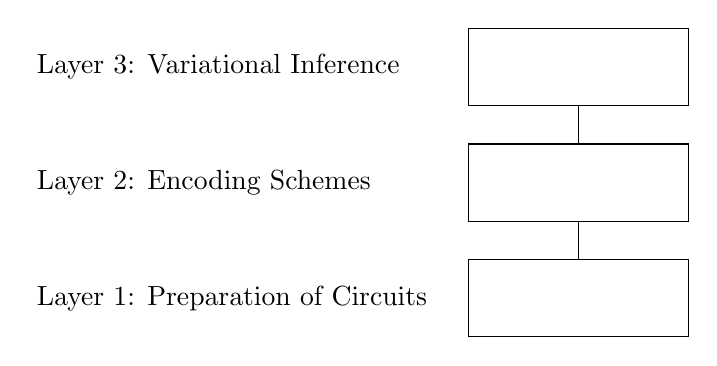
\begin{tikzpicture}[scale=0.35,yscale=0.7]
    \draw (-10,10) rectangle (-2,14);
    \node [anchor=center] at (-6,12) {\spreasoning{}};
    \node [anchor=west] at (-26,12) {Layer 3: Variational Inference};

    \draw (-6,10) -- (-6,8);
    \draw (-10,4) rectangle (-2,8);
    \node [anchor=center] at (-6,6) {\sprepresentation{}};
    \node [anchor=west] at (-26,6) {Layer 2: Encoding Schemes};

    \draw (-6,4) -- (-6,2);
    \draw (-10,-2) rectangle (-2,2);
    \node [anchor=center] at (-6,0) {\spengine{}};
    \node [anchor=west] at (-26,0) {Layer 1: Preparation of Circuits};
\end{tikzpicture}
\end{center}

\subsection{Generic Contraction}

So far, the generic contraction routine consists in activation circuits preparing for each tensor an ancilla variable, and post-selecting the measurements where the ancilla variable is $1$.
The resulting tensor of the contraction is a $\mathrm{PandasCore}$ storing the post-selected measurement results in a dataframe.